\documentclass{article}
\usepackage[utf8]{inputenc}
\usepackage{graphicx}
\usepackage{geometry}
\usepackage{fancyhdr}

\geometry{
  a4paper,
  total={170mm,230mm},
  left=20mm,
  top=3.5cm,
}

% Make sure the header has enough vertical room
\setlength{\headheight}{20pt}
\setlength{\headsep}{20pt}

% Define your header/footer once
\fancypagestyle{fancy}{
  \fancyhf{}
  \fancyhead[L]{Week 2 Assignment}
  \fancyhead[R]{\authorname}         % see \newcommand below
  \fancyfoot[L]{\today}              % use \today or your own date macro
  \fancyfoot[R]{
\includegraphics[width=2cm]{NAU_ctr_282_3514_150.png}}
}

% Make "plain" pages match "fancy" (covers first page, chapter starts, etc.)
\fancypagestyle{plain}{
  \fancyhf{}
  \fancyhead[L]{Week 2 Assignment}
  \fancyhead[R]{\authorname}
  \fancyfoot[L]{\today}
  \fancyfoot[R]{
\includegraphics[width=2cm]{NAU_ctr_282_3514_150.png}}
}

% Activate globally
\pagestyle{fancy}

% (Optional) define a clean author macro for header use
\newcommand{\authorname}{Stephen Nuno} % or pull from \author with \makeatletter if you prefer


 \usepackage{graphicx}
 \usepackage{titling}
 \usepackage{float}

 \title{Week 2 Assignment: Including references using biblatex
}
\author{Stephen A. Nu\~no} %Add your name here
\date{September 2, 2025}
 


\makeatletter
\def\@maketitle{%
  \newpage
  \null
  \vskip 1em%
  \begin{center}%
  \let \footnote \thanks
    {\LARGE \@title \par}%
    \vskip 1em%
    %{\large \@date}%
  \end{center}%
  \par
  \vskip 1em}
\makeatother

\usepackage{lipsum}  
\usepackage{cmbright}

%The packages below enables the use of in-text citations and citations using the MLA format.
%\usepackage[style=mla, backend=biber]{biblatex}
%\usepackage{csquotes}
%\addbibresource{samplebiblatex.bib}


%If you want to use the APA format, you would use the following packages instead. 

\usepackage[style=apa, backend=biber]{biblatex} 
\DeclareLanguageMapping{american}{american-apa} 
\usepackage{csquotes} 
\addbibresource{myreferences.bib}


\begin{document}

\maketitle

\noindent\begin{tabular}{@{}ll}
    Name & \theauthor\\
    Student ID. &  xxx-xx-xxx\\ %Add your Student ID# here
    Due Date: &  September 4, 2025; before class
\end{tabular}

\section*{Introduction}

This is a short assignment allowing you to practice using the citation commands to create a references page from the sources you are using for a research paper. Below are some important components of a bibliography. The following are the packages you would use if you wanted to format your citations into MLA format. You will need to use the following packages in your preamble: 

\begin{itemize}
    \item \verb|\usepackage[style=mla, backend=biber]{biblatex}|
    \item \verb|\usepackage{csquotes}|
    \item \verb|\addbibresource{myreferences.bib}| \textbf{You will add your .bib file to this command, telling Overleaf where your references are. Here is it called ``myreferences.bib". }
\end{itemize}

\textbf{If you want to use the APA style format, you would use the following packages instead: 
}
\begin{itemize}
    \item \verb|\usepackage[style=apa, backend=biber]{biblatex} |
    \item \verb|\DeclareLanguageMapping{american}{american-apa} |
    \item \verb|\usepackage{csquotes}|
    \item \verb|\addbibresource{references.bib}| \textbf{\textit{Note that the name of the .bib file in this assignment is ``myreferences.bib". This is the file you will replace from your Zotero.}}
\end{itemize}

\section*{Commands you will be using for this exercise}

Next, you will be using the following commands throughout the assignment: 

\begin{itemize}
    \item \verb|\parencite{}| \textbf{This command forces parentheses in your citation.}
    \item \verb|\cite{}| Standard \textbf{citation depending on which format you use. }
    \item \verb|\textcite{}| \textbf{This cites a references in the text of your sentence.}
    \item \verb|\printbibliography| \textbf{This adds your references in alphabetical order wherever your place the command.}
\end{itemize}

\section*{MLA Examples}

Below is an example of the different formats using the ``MLA style": 

\begin{itemize}
    \item \verb|\parencite{villa2020,zapata2019}|\textrightarrow\textbf{(Villa; Zapata)}
    \item \verb|\cite{villa2020}|\textrightarrow\textbf{(Villa)} \textit{Note: same as above, since MLA defaults to parenthetical}
    \item \verb|\cite{villa2020,zapata2019}| \textrightarrow \textbf{(Villa; Zapata)} 
    \item \verb|\textcite{villa2020,zapata2019}|\textrightarrow Doe and Smith argue that…
    \item \verb|\parencite[23]{villa2020}|
    \item \verb|\parencite[45]{zapata2019}| \textrightarrow If you want to cite pages, MLA will format them as: \textbf{(Villa 23; Zapata 45)}
\end{itemize}

\section*{APA Examples}
Below is an example of the different formats using the ``APA style" 

\begin{itemize}
    \item \verb|\parencite{villa2020,zapata2019}|\textrightarrow\textbf{(Villa, 2019; Zapata, 2020)}
    \item \verb|\cite{villa2020}|\textrightarrow \textbf{Villa (2020)} 
    \item \verb|\textcite{villa2020,zapata2019}|\textrightarrow \textbf{Villa (2020) and Zapata (2019) argue that…}
    \item \verb|\parencite[23]{villa2020}|
    \item \verb|\parencite[45]{zapata2019}| \textrightarrow If you want to cite pages, APA will format them as: \textbf{(Villa, 2020, p. 23; Zapata, 2019, p. 45)}
\end{itemize}

\section*{Exercise}
\begin{enumerate}
    \item Open your Zotero and make sure the references you added have the citation information for each article filled out accurately.
    \begin{figure} [H]
        \centering % puts the image in the horizontal centre of the page
        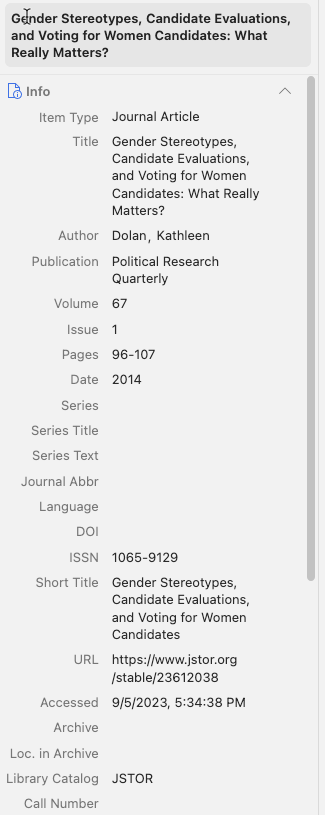
\includegraphics[width = 4cm]{dolan_info.png} 
\end{figure}

\newpage
    \item Highlight your sources and right-click to export the references you collected into a "Biblatex" file. Name your file whatever you want, "references" or "citations" are fine. That file will be saved as a .bib file. 

    \begin{figure} [H]
        \centering % puts the image in the horizontal centre of the page
        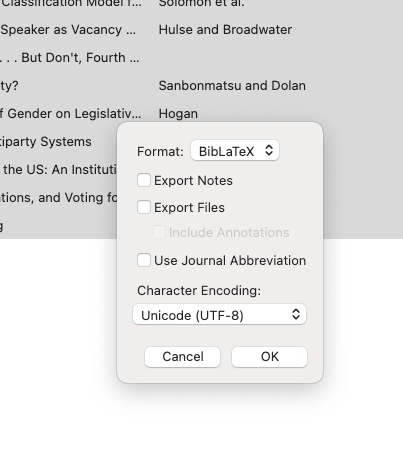
\includegraphics[width = 8cm]{biblatex pic.png} 
    \end{figure}
    \item Upload your .bib file into your Overleaf library.
    \item Add the name of your file to the \verb|\addbibresource{}| command above. For example if you named your file ``references" the command would look like \verb|\addbibresource{references.bib}|. Now you can use the citation commands!
    \item Write a short summary of ten of your references. It is ok to cut and paste from the abstract. I will give you an example below. 
\end{enumerate}

\newpage
\section*{Working Bibliography Exercise}
\textbf{EXAMPLE}

I included a picture of the reference in Figure \ref{fig:dolan} below that I am using in the example. You do not need to include a picture. I just want you to see it as an illustration. 
\begin{figure} [H]
    \centering % puts the image in the horizontal centre of the page
    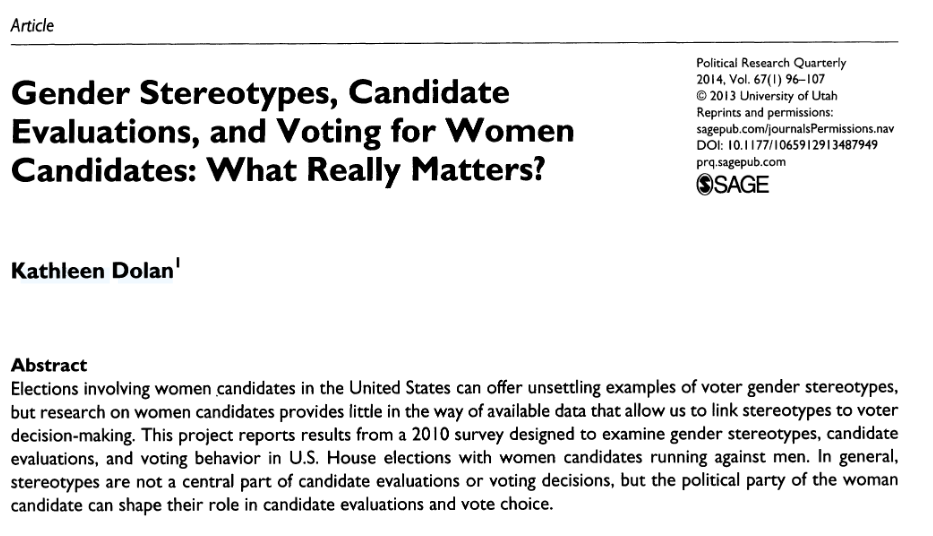
\includegraphics[width = 10cm]{dolan.png} 
    \caption{Dolan Article} % this prints the caption below the figure
    \label{fig:dolan} % this internally labels the figure for future referencing.
\end{figure}

\begin{enumerate}
    \item In ``Gender Stereotypes, Candidate Evaluations, and Voting for Women Candidates: What Really Matter?", \textcite{dolan_gender_2014} argues that research on women candidates provides little in the way of available data that allow us to link stereotypes to decision-making.
    \item Research shows that stereotypes are not a central part of candidate evaluations or voting decisions, but the political party of the woman candidate can shape their role in candidate evaluations and vote choice \parencite{dolan_gender_2014}.
\end{enumerate}

\textbf{Now your turn.} Write two short summaries for 10 of your references using the \verb|\textcite| command and the \verb|\parencite| command. Use the command I included below to add your references just like I did above. I have already included the \verb|\printbibliograph| command with an addition option to name your bibliography "Works Cited". It should compile automatically once you start adding your in-text and parenthetical citations.

\newpage
\section*{My Working Bibliography}

\textbf{Reference \# 1}

\begin{enumerate}
    \item Add your \textbf{first} reference here using \verb|\textcite| command.
    \item Add your \textbf{first} reference here using \verb|\parencite| command.
\end{enumerate}

\textbf{Reference \# 2}

\begin{enumerate}
    \item Add your \textbf{second} reference here using \verb|\textcite| command.
    \item Add your \textbf{second} reference here using \verb|\parencite| command. 
\end{enumerate}

\textbf{Reference \# 3}

\begin{enumerate}
    \item and so on \ldots
    \item and so on \ldots
\end{enumerate}

\textbf{Reference \# 4}

\begin{enumerate}
    \item and so on \ldots
    \item and so on \ldots
\end{enumerate}

\textbf{Reference \# 5}

\begin{enumerate}
    \item and so on \ldots
    \item and so on \ldots
\end{enumerate}

\textbf{Reference \# 6}

\begin{enumerate}
    \item and so on \ldots
    \item and so on \ldots
\end{enumerate}

\textbf{Reference \# 7}

\begin{enumerate}
    \item and so on \ldots
    \item and so on \ldots
\end{enumerate}

\textbf{Reference \# 8}

\begin{enumerate}
    \item and so on \ldots
    \item and so on \ldots
\end{enumerate}

\textbf{Reference \# 9}

\begin{enumerate}
    \item and so on \ldots
    \item and so on \ldots
\end{enumerate}

\textbf{Reference \# 10}

\begin{enumerate}
    \item and so on \ldots
    \item and so on \ldots
\end{enumerate}

\newpage

%the command below will print out your bibliography. 
\printbibliography[title={Works Cited}] % Not that adding [title={Works Cited}] as an option to the \printbibliography command changes the title from References to Works Cited.
\end{document}
